\documentclass{article}
\usepackage[english]{babel}
\usepackage[utf8]{inputenc}
\usepackage{fancyhdr}
\usepackage{amsmath}
\usepackage{pdfpages}
\usepackage{graphicx}
\graphicspath{ {./images/} }

\pagestyle{fancy}
\fancyhf{}
\rhead{CS760}
\lhead{Cheng-Wei Lu}
\rfoot{Page \thepage}

\begin{document}

\section*{CS 760 Homework 3 by Cheng-Wei Lu}

\subsection*{Problem 3.1}
\subsubsection*{(a)}
	I set the iteration number of $\hat{\theta}$ update to 1000. Step size = 1/20. I change the step size by multiply it with 3/4 every 50 iterations. The stop criteria is that when iteration number reaches 1000 or when the improvement for likelihood is less than $10^(-3)$, the parameter update will stop.

\subsubsection*{(b)}
	It took about 18 seconds for my computer to converge.
\subsubsection*{(c)}
	\begin{equation*}
		\hat{\theta} =  \begin{pmatrix} 1.802\text{(class 1)}\\ 0.567 \text{(class 2)}\\ -0.645 \text{(class 3)}\\ 2.769 \text{(sex)}\\ -1.372\text{(age)}\\ -0.217\text{(siblings/spouses aboard)}\\-0.041\text{(parents/children aboard)}\\ 0.079\text{(fare)}\\-0.274\text{(intercept)} \end{pmatrix} 	\end{equation*}
	
\subsubsection*{(d)}
	likelihood $ = -390.5596 $
	
\subsubsection*{(e)}
	The distribution of $\hat{\theta}$ is $N(\theta^*, \frac{1}{N}I^{-1}_{\theta^{*}})$, where the $\theta^*$ is the real $\theta$ and the variance is represented by a covariance matrix $\frac{1}{N}I^{-1}_{\theta^{*}}$, which is of the following  value :
	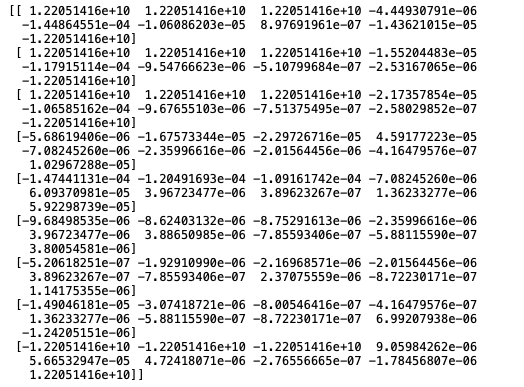
\includegraphics[scale=0.5]{fisher}
	
\subsection*{Problem 3.2}
\subsubsection*{(a)}
	By the invariance property of MLE, we know that  $\hat{w} = x^T\hat{\theta}$.
\subsubsection*{(b)}
	Since  $\hat{\theta}  \xrightarrow[]{d} N(\theta^*, \frac{1}{N}I^{-1}_{\theta^{*}})$, and $\hat{w} = x^T\hat{\theta}$. It implies  $\hat{w}  \xrightarrow[]{d} N(\theta^*, \frac{1}{N}x^{T}I^{-1}_{\theta^{*}}x)$.

	 

\end{document}

